\documentclass[compress]{beamer}
%
% Choose how your presentation looks.
%
% For more themes, color themes and font themes, see:
% http://deic.uab.es/~iblanes/beamer_gallery/index_by_theme.html
%
\mode<presentation>
{
	\usetheme{Dresden}      % or try Darmstadt, Madrid, Warsaw, ...  
	%\useoutertheme{infolines} % split, tree, infolines
	%\useinnertheme{rectangles}
	\usecolortheme{orchid} % or try albatross, beaver, crane, ...
	\usefonttheme{structuresmallcapsserif}  % or try serif, structurebold, ...
	\setbeamertemplate{navigation symbols}{}
	\setbeamertemplate{caption}[numbered]
	\setbeamertemplate{footline}[frame number]
} 

\usepackage[english]{babel}
\usepackage[utf8x]{inputenc}
\usepackage{tikz}
\usetikzlibrary{trees,snakes,arrows}
\usepackage{tabularx}
\usepackage{subfig}
\usepackage{graphicx}
%\usepackage{animate}

\def\tobar{\mathrel{\mkern3mu  \vcenter{\hbox{$\scriptscriptstyle+$}}%
		\mkern-12mu{\to}}}

\title[BA Hobbhahn 2019]{Object Detection using the Scattering Transform}
\author{Marius Hobbhahn}
\date{\today}

\begin{document}
	
	\begin{frame}
		\titlepage
	\end{frame}
	%
	% Uncomment these lines for an automatically generated outline.
	%\begin{frame}{Outline}
	%  \tableofcontents
	%\end{frame}
	%
	\section{Introduction}
	\subsection{ } % for the dots - there most probably is a more elegant solution.
	%
	\begin{frame}{Object Detection}
		\begin{figure}
			\begin{tabular}{ccc}
				\subfloat[]{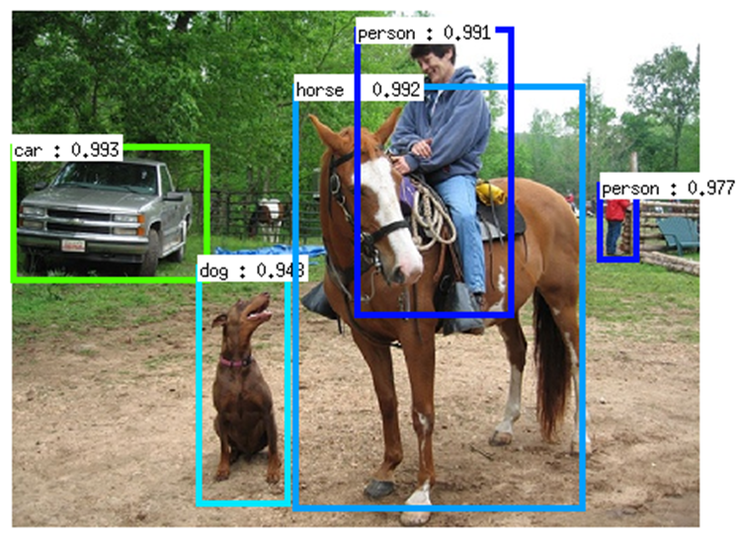
\includegraphics[height=2.5cm]{images/casual_scene_with_annots.png}} 
				& \subfloat[]{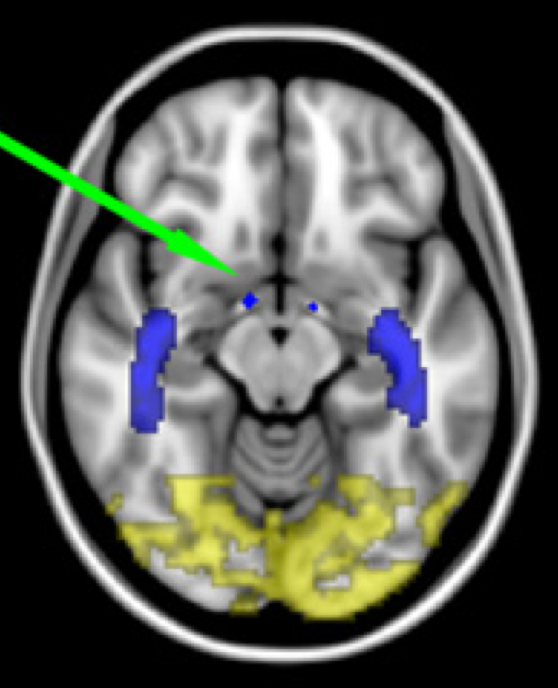
\includegraphics[height=2.5cm]{images/brain_imaging.png}} 
				&
				\subfloat[]{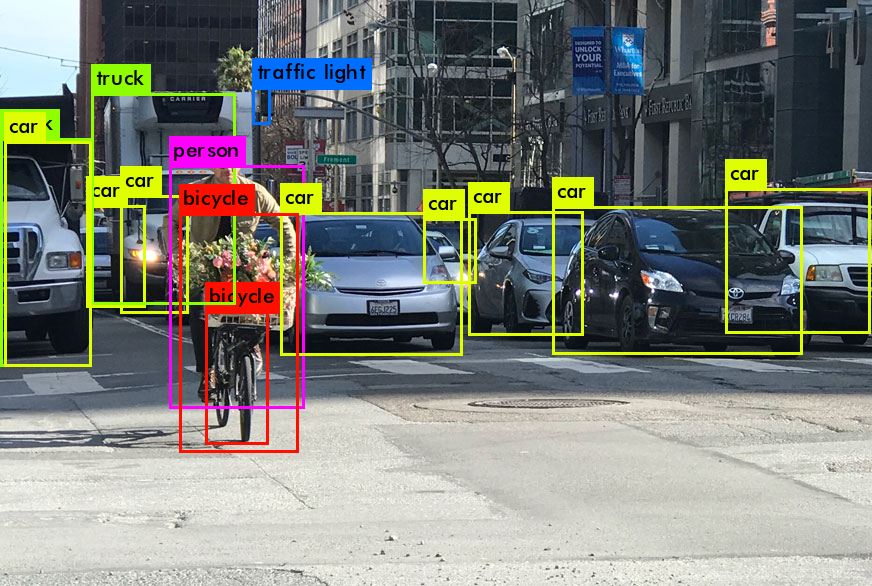
\includegraphics[height=2.5cm]{images/example_traffic_scene_with_annots.png}}\\
			\end{tabular}
		\end{figure}
		\begin{itemize}
			\item Automatic annotation of everyday photos
			\item Brain disease recognition
			\item Traffic scene detection
		\end{itemize}
		
	\end{frame}
	%
	\begin{frame}{Motivation}
		\begin{block}{Problems}
			\begin{enumerate}
				\item Loads of data necessary for training
				\item Capability to generalize unclear for different circumstances (i.e. invariances w.r.t. many things)
			\end{enumerate}
		\end{block}
		\begin{block}{Possible solutions}
			\begin{enumerate}
				\item Filters that generalize quickly
				\item Theoretical bounds for some invariances (i.e. translation, location)
			\end{enumerate}
		\end{block}
	\end{frame}
	%
	\begin{frame}{Scattering Transform}
		\begin{block}{Basic Idea}
			Static image filter that has certain theoretical guarantees with respect to invariances (i.e. location, scale, rotation).
		\end{block}
		\begin{equation}
		\psi(u) = C_1 (e^{iu.\xi} - C_2) e^{\frac{-|u|^2}{2\sigma^2}}
		\label{eq:morlet2d}
		\end{equation}
		\begin{figure}[!htb]
			\centering
			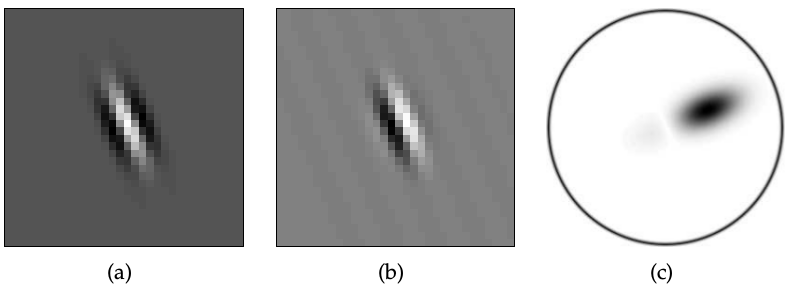
\includegraphics[width = 0.75\textwidth]{images/morlet2d.png}
			\caption{Complex morlet wavelet. a) Real part of $\psi$. b) Imaginary part of $\psi$. c) Fourier modulus $|\hat{\psi}|$.}
			\label{fig:morlet2d}
		\end{figure}
	\end{frame}
	%
	%what is U
	%what is f
	%what is \phi
	%what is S
	%what is \lambda
	%
	\begin{frame}{Visualization of the filter bank}
		\begin{figure}[!htb]
			\centering
			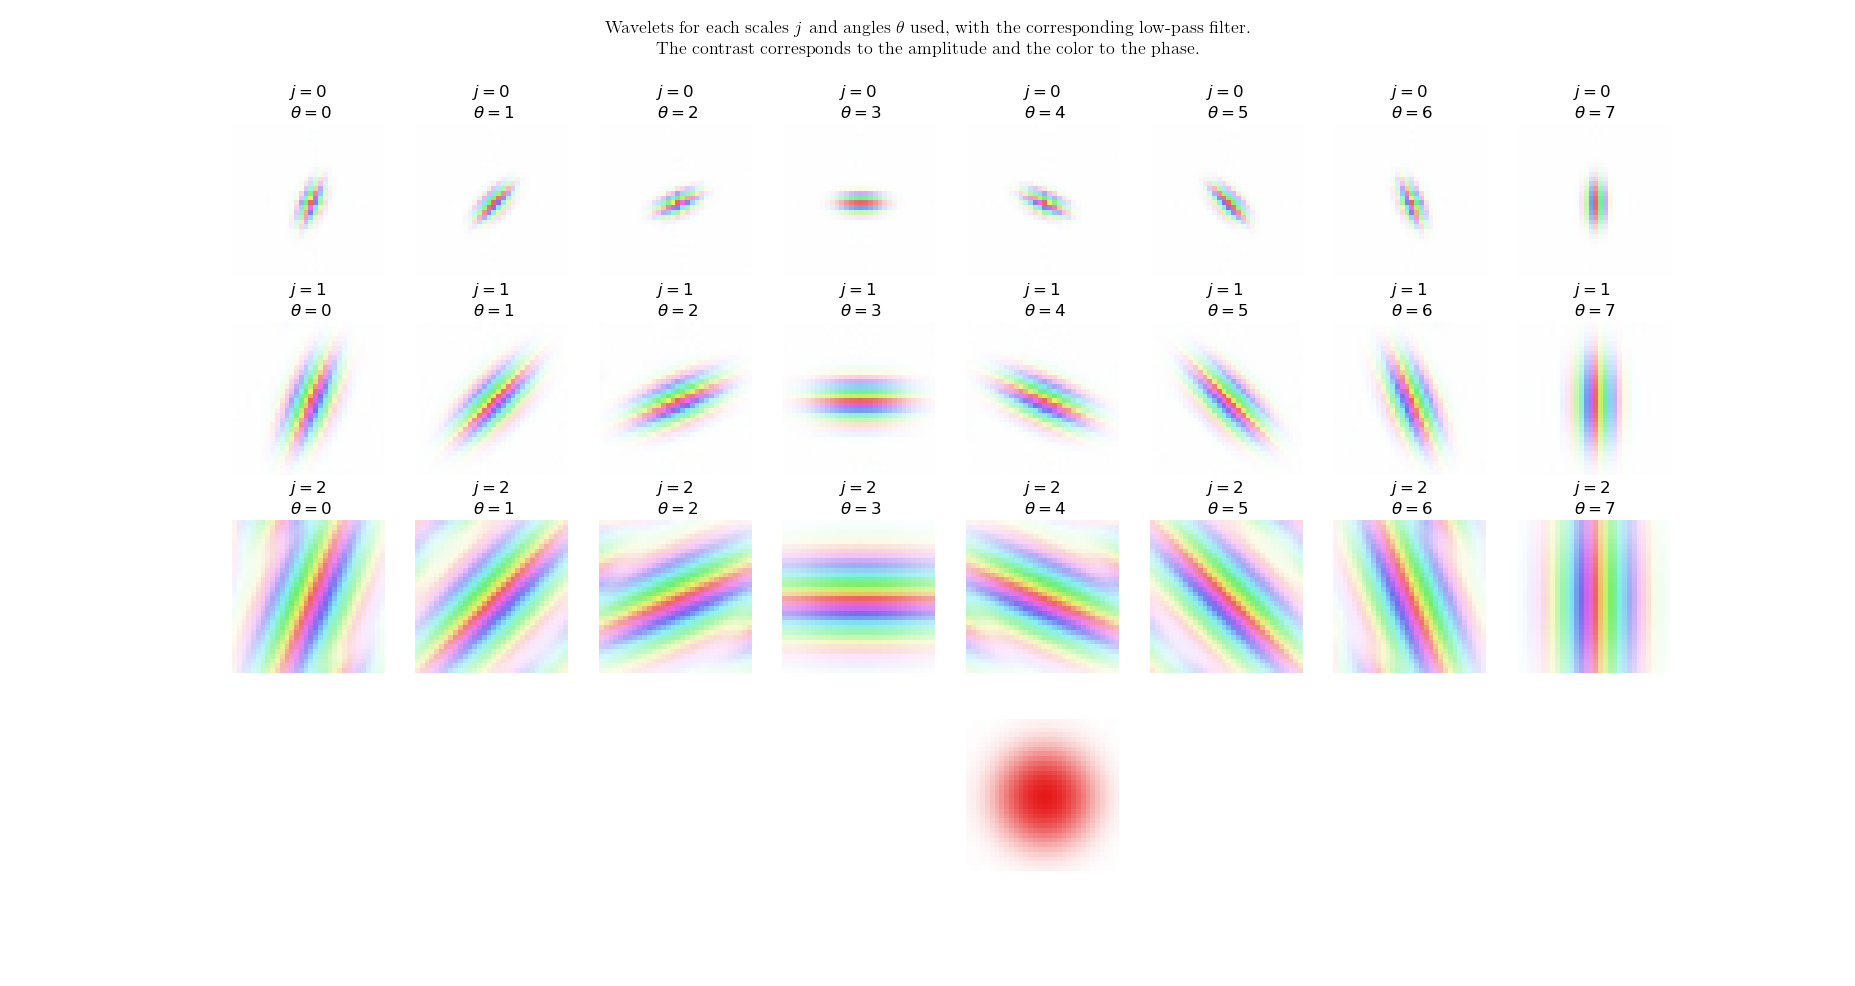
\includegraphics[width=\textwidth]{images/filter_bank_vis.png}
			\caption{Visualization of the filter bank}
			\label{fig:viz_filter_bank}
		\end{figure}
	\end{frame}
	%
	\begin{frame}{Scattering Networks}
		\begin{block}{Basic Idea}
			Apply the scattering transform multiple times to get higher order scattering coefficients.
		\end{block}
		\begin{figure}[!htb]
			\centering
			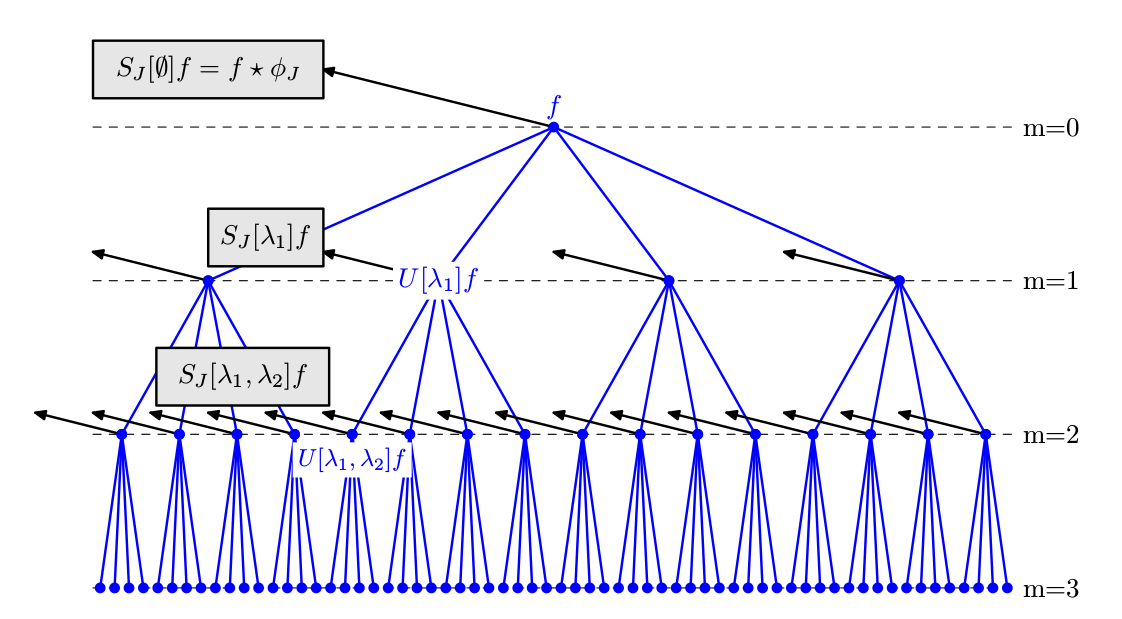
\includegraphics[width = 0.75\textwidth]{images/scattering_network.png}
			\caption{}
			\label{fig:scattering_network}
		\end{figure}
	\end{frame}
	%
	\begin{frame}{Visualization of the scattering coefficients}
		\begin{figure}[!htb]
			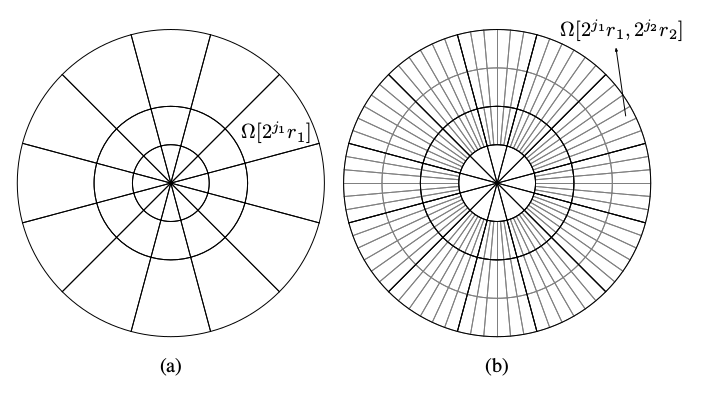
\includegraphics[width=0.8\textwidth]{images/viz_scattering_coeff_m12.png}
			\caption{Visualization of the scattering coefficients for m=1 (left) and m=2 (right)}
		\end{figure}
	\end{frame}
	%
	\begin{frame}{Example of the scattering coefficients}
		\begin{figure}[!htb]
			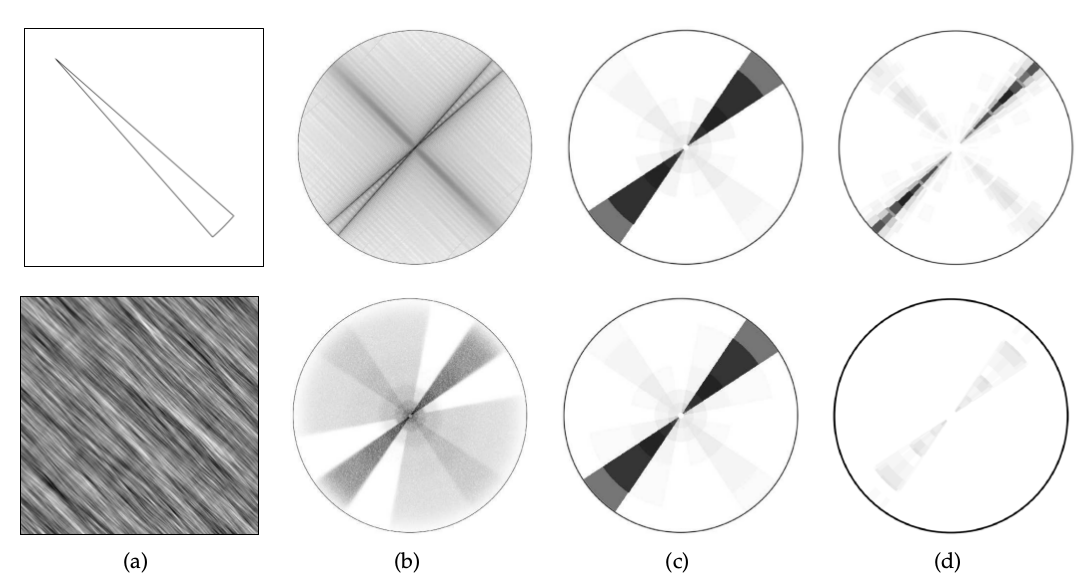
\includegraphics[width=0.8\textwidth]{images/scattering_coefficients_example.png}
			\caption{Scattering display of two images having the same first order scattering coefficients. a) Image, b) Fourrier modulus c) Coefficients with m=1, d) Coefficients with m=2}
		\end{figure}
	\end{frame}
	%
	\begin{frame}{Hybrid scattering networks}
		\begin{figure}
			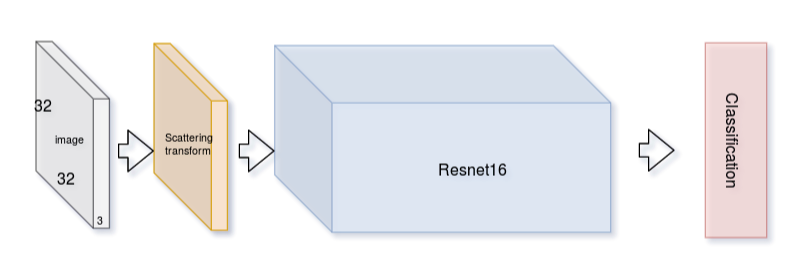
\includegraphics[width=0.9\textwidth]{images/arch_hybrid_scattering_CIFAR10.png}
			\caption{Architecture}
		\end{figure}
		\begin{figure}
			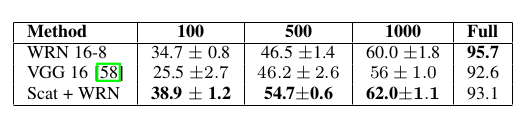
\includegraphics[width=0.9\textwidth]{images/results_hybrid_scattering_CIFAR10.png}
			\caption{Results of 2017 paper}
		\end{figure}
	\end{frame}
	%
	\begin{frame}{Datasets - Kitti}
		\begin{block}{kitti}
			\begin{itemize}
				\item Content: street and traffic scenes
				\item number of samples: 7480
			\end{itemize}			
		\end{block}
		\begin{figure}
			\centering
			\begin{tabular}{cc}
				\subfloat[]{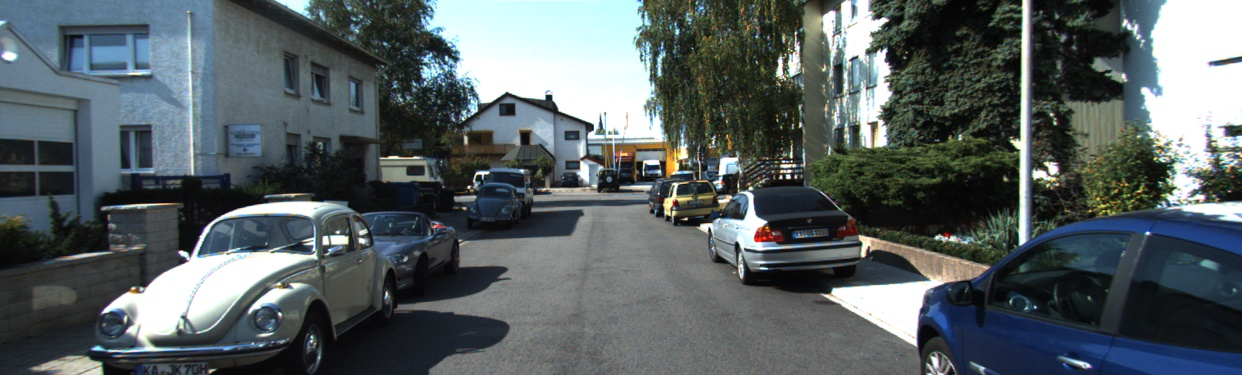
\includegraphics[width=5cm]{images/kitti_sample_1.jpg}} 
				& \subfloat[]{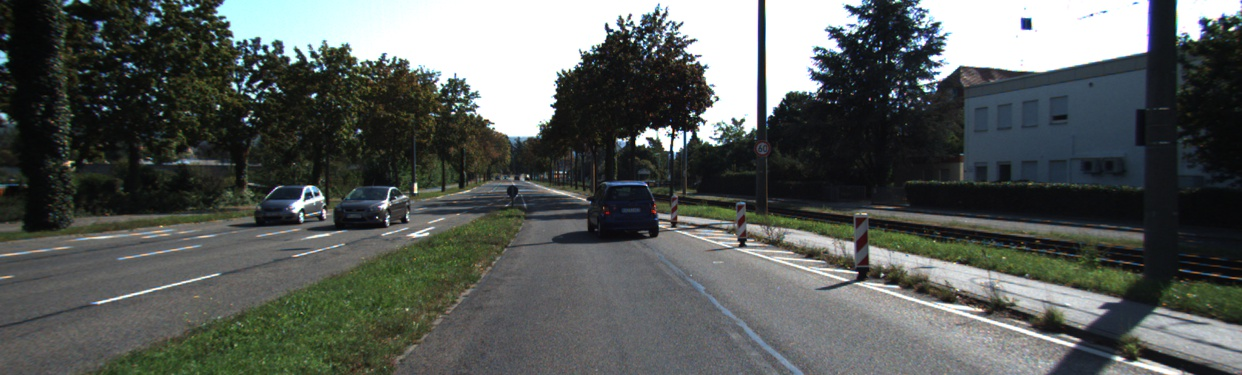
\includegraphics[width=5cm]{images/kitti_sample_2.jpg}} \\
				\subfloat[]{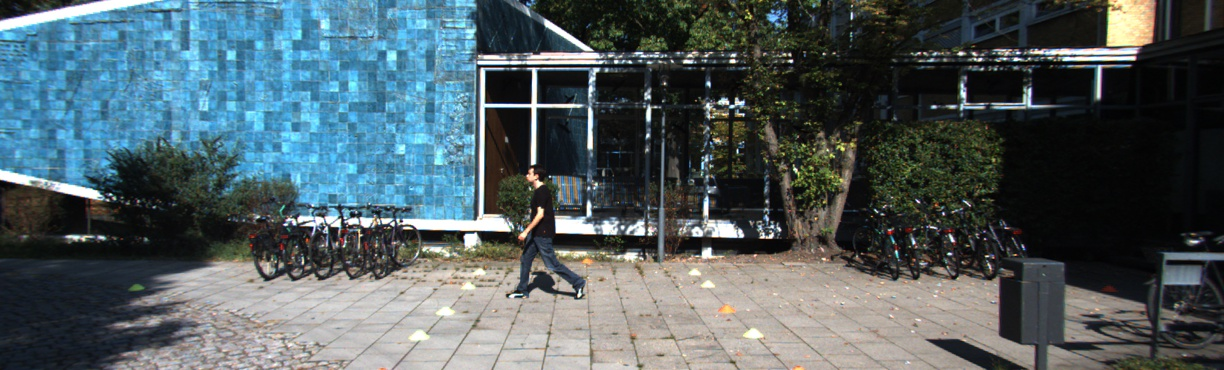
\includegraphics[width=5cm]{images/kitti_sample_3.jpg}} 
				& \subfloat[]{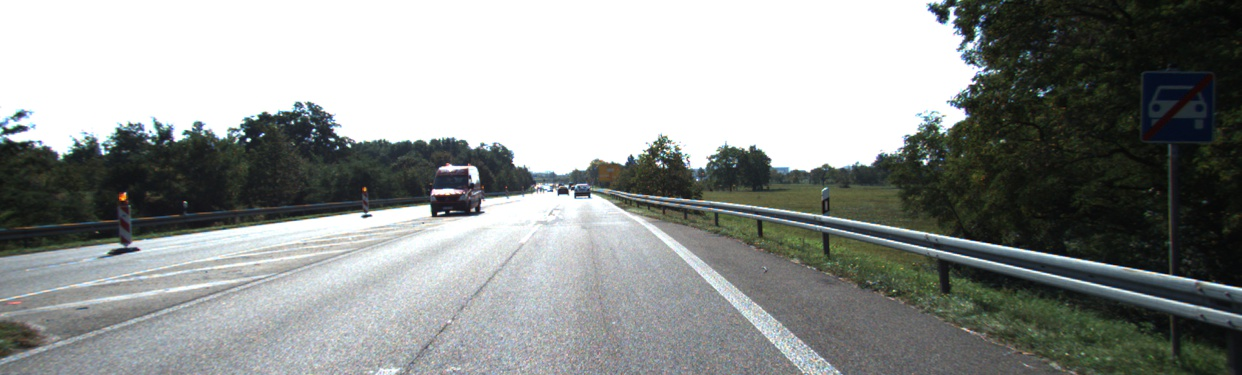
\includegraphics[width=5cm]{images/kitti_sample_4.jpg}} 
			\end{tabular}
		\end{figure}
	\end{frame}
	%
	\begin{frame}{Datasets - VOC}
		\begin{block}{VOC}
			\begin{itemize}
				\item miscellaneous (singular) objects
				\item VOC2007 and VOC2012
				\item number of samples: 9963 + 17125
			\end{itemize}
		\end{block}
		\begin{figure}
			\centering
			\begin{tabular}{ccc}
				\subfloat[]{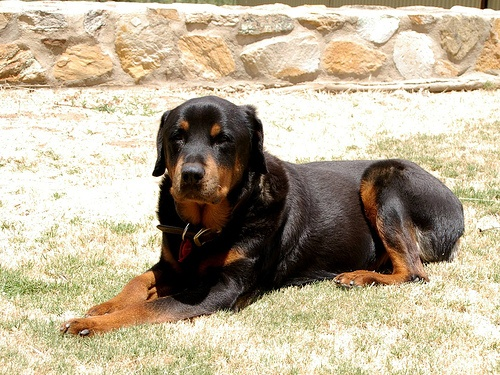
\includegraphics[width=3cm]{images/VOC_sample_1.jpg}} 
				& \subfloat[]{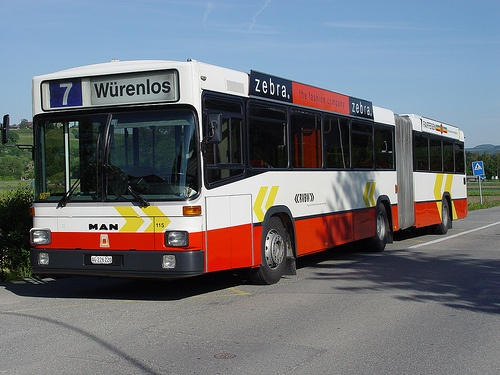
\includegraphics[width=3cm]{images/VOC_sample_2.jpg}}&
				\subfloat[]{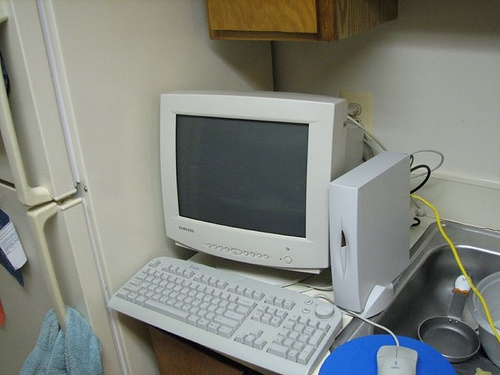
\includegraphics[width=3cm]{images/VOC_sample_3.jpg}}
			\end{tabular}
		\end{figure}
	\end{frame}
	%
	\section{Models/Experiments}
	\subsection{ } % for the dots - there most probably is a more elegant solution.
	\begin{frame}{Simple Single Shot MultiBox Detector (SSD)}
		\begin{figure}
			\centering
			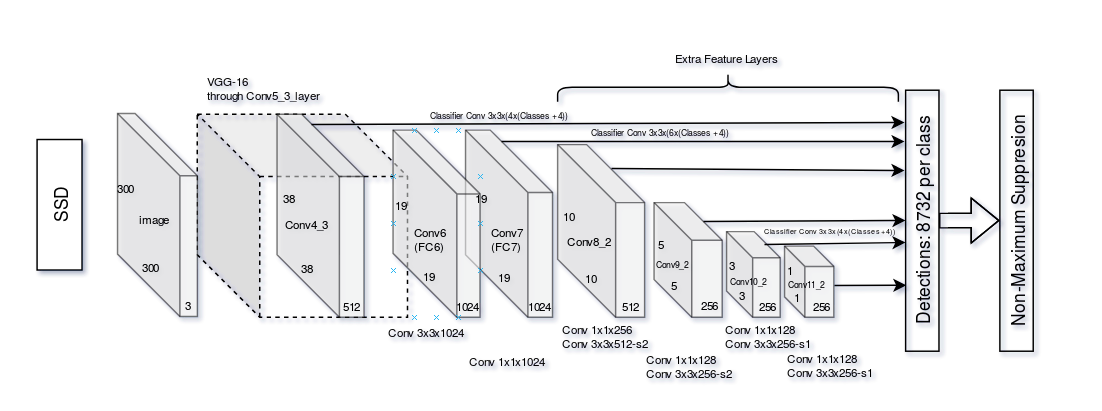
\includegraphics[width=\textwidth]{images/simple_ssd.png}
		\end{figure}
	\end{frame}
	%
	\begin{frame}{Sequential Scattering SSD}
		\begin{block}{}
			\begin{itemize}
				\item Scattering is applied before data is piped through SSD
			\end{itemize}
		\end{block}
		\begin{figure}
			\centering
			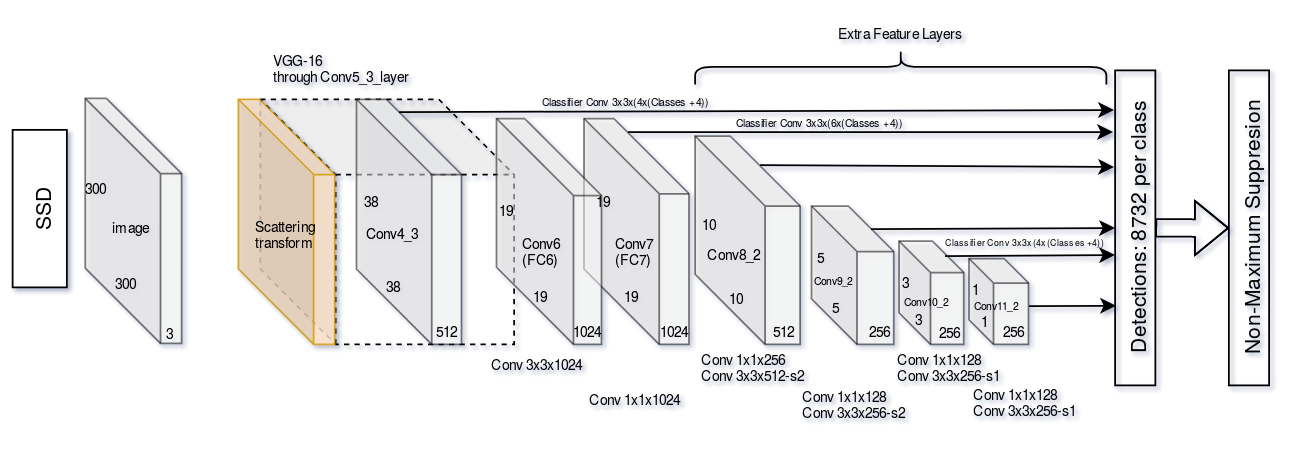
\includegraphics[width=\textwidth]{images/sequential_scattering_ssd.png}
		\end{figure}
	\end{frame}
	%
	\begin{frame}{Continuous Fusion Scattering SSD}
		\begin{block}{}
			\begin{itemize}
				\item Data is piped through scattering and standard SSD and continuously merged at different stages
			\end{itemize}
		\end{block}
		\begin{figure}
			\centering
			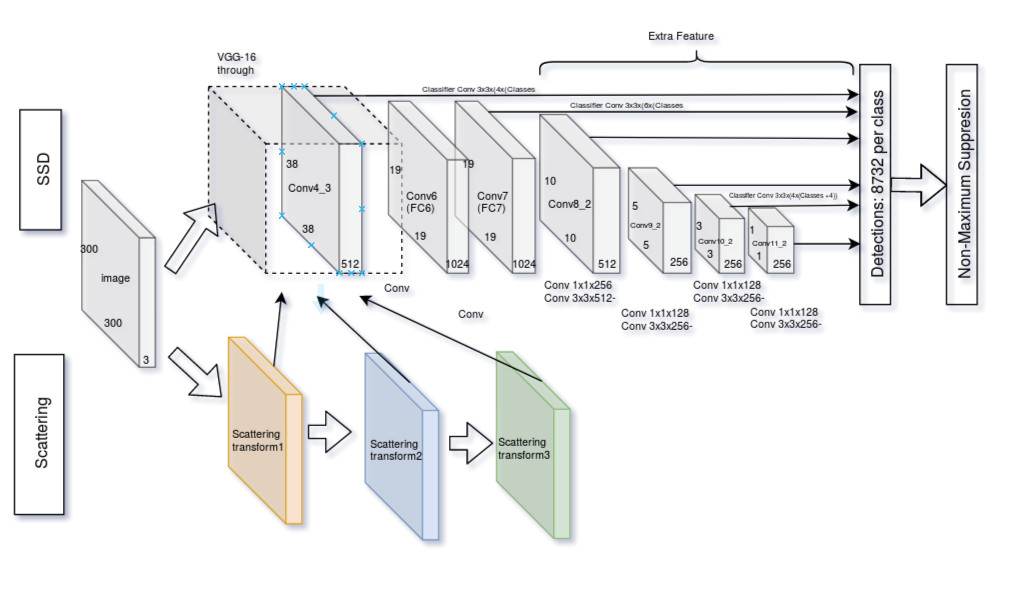
\includegraphics[width=0.8\textwidth]{images/parallel_scattering_ssd.png}
		\end{figure}
	\end{frame}
	%
	\begin{frame}{Furthers plans and additional ideas}
		\begin{itemize}
			\item try to achieve same baseline as other SSD implementations on kitti did: $\sim$ 50\%
			\item use other base-architecture: faster RCNN, masked RCNN, ...
			\item integrate further datasets: COCO, FDDB, ...
		\end{itemize}
	\end{frame}
	%
	\begin{frame}{Status Quo in pictures - Kitti}
		\begin{figure}
			\centering
			\begin{tabular}{c}
				\subfloat[]{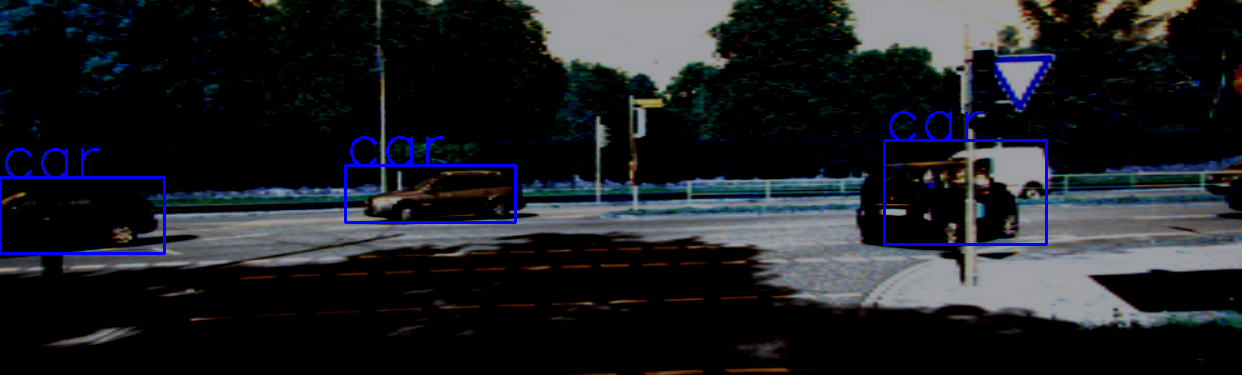
\includegraphics[width=10cm]{images/test_OK.png}}  \\
				\subfloat[]{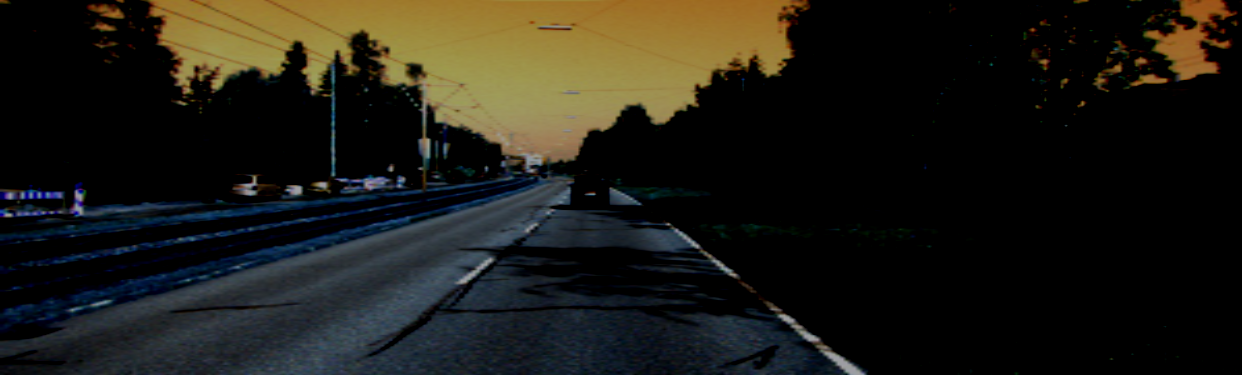
\includegraphics[width=10cm]{images/test_Bad.png}} 
			\end{tabular}
		\end{figure}
	\end{frame}
	%
	\begin{frame}{Status Quo in pictures - VOC + scattering}
		\begin{figure}
			\centering
			\begin{tabular}{c c}
				\subfloat[]{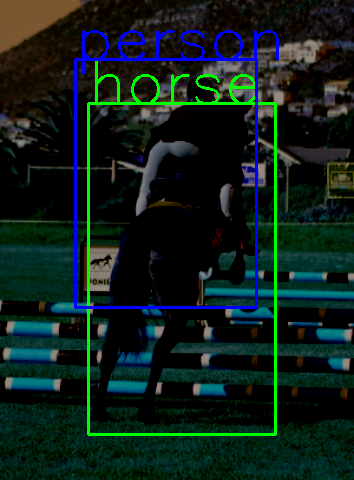
\includegraphics[width=4cm]{images/test_VOC.png}} &
				\subfloat[]{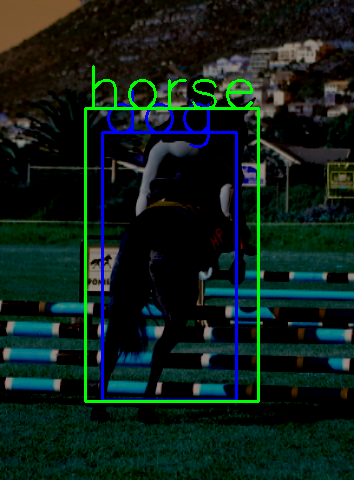
\includegraphics[width=4cm]{images/horse_dog_pres.png}}  
			\end{tabular}
		\end{figure}
	\end{frame}
	%
	\begin{frame}{Status Quo in numbers}
		\begin{tabular}{l | c | c }
			dataset & train accuracy & test accuracy \\ \hline
			VOC & 0.76 & 0.61 \\
			Kitti & 0.82 & 0.12\\
			kitti1000x300 & - & 0.05 \\
			Kitti small & 0.95 & 0.0 \\
			Kitti small1000x300 & 0.95 & 0.0 \\			
			Scattering Hybrid VOC & - & 0.06 
		\end{tabular}
	\end{frame}
	%
	\section{Outro}
	\subsection{ } % for the dots - there most probably is a more elegant solution.
	\begin{frame}{Questions and Suggestions}
		\begin{itemize}
			\item Any questions?
			\item Any suggestions, tips, ... are very welcome
		\end{itemize}
	\end{frame}
	%
	\begin{frame}[shrink=30]{References}
		\cite{scatteringTransform2012}, \cite{InvariantScatteringTextureDiscrimination2013}, \cite{DeepRotoTranslation2014}, 
		\cite{ScalingTheScatteringTransform2017},
		\cite{3DScatteringTransformNeuro2017}
		\bibliographystyle{alpha}
		\small\bibliography{bibliography}
	\end{frame}
	

\end{document}
